\section{Question 1: Experimental Results and Analysis}

\subsection{Quantitative Performance}

Table~\ref{tab:q1-main} reports test-set performance for the two from-scratch models on \texttt{emails\_2.csv}.

\begin{table}[H]
\centering
\caption{Question 1 test metrics on \texttt{emails\_2.csv}}
\label{tab:q1-main}
\begin{tabular}{lcc}
\toprule
Metric & Logistic Regression & Naive Bayes \\
\midrule
Accuracy  & 0.9633 & 0.9420 \\
Precision & 0.9199 & 0.8681 \\
Recall    & 0.9567 & 0.9433 \\
F1-score  & 0.9379 & 0.9042 \\
\bottomrule
\end{tabular}
\end{table}

Logistic Regression outperforms Naive Bayes on every metric. The largest practical gain appears in precision and F1-score, suggesting fewer false positives while preserving strong detection of spam emails.

\subsection{Confusion and Ranking Behavior}

\begin{figure}[H]
\centering
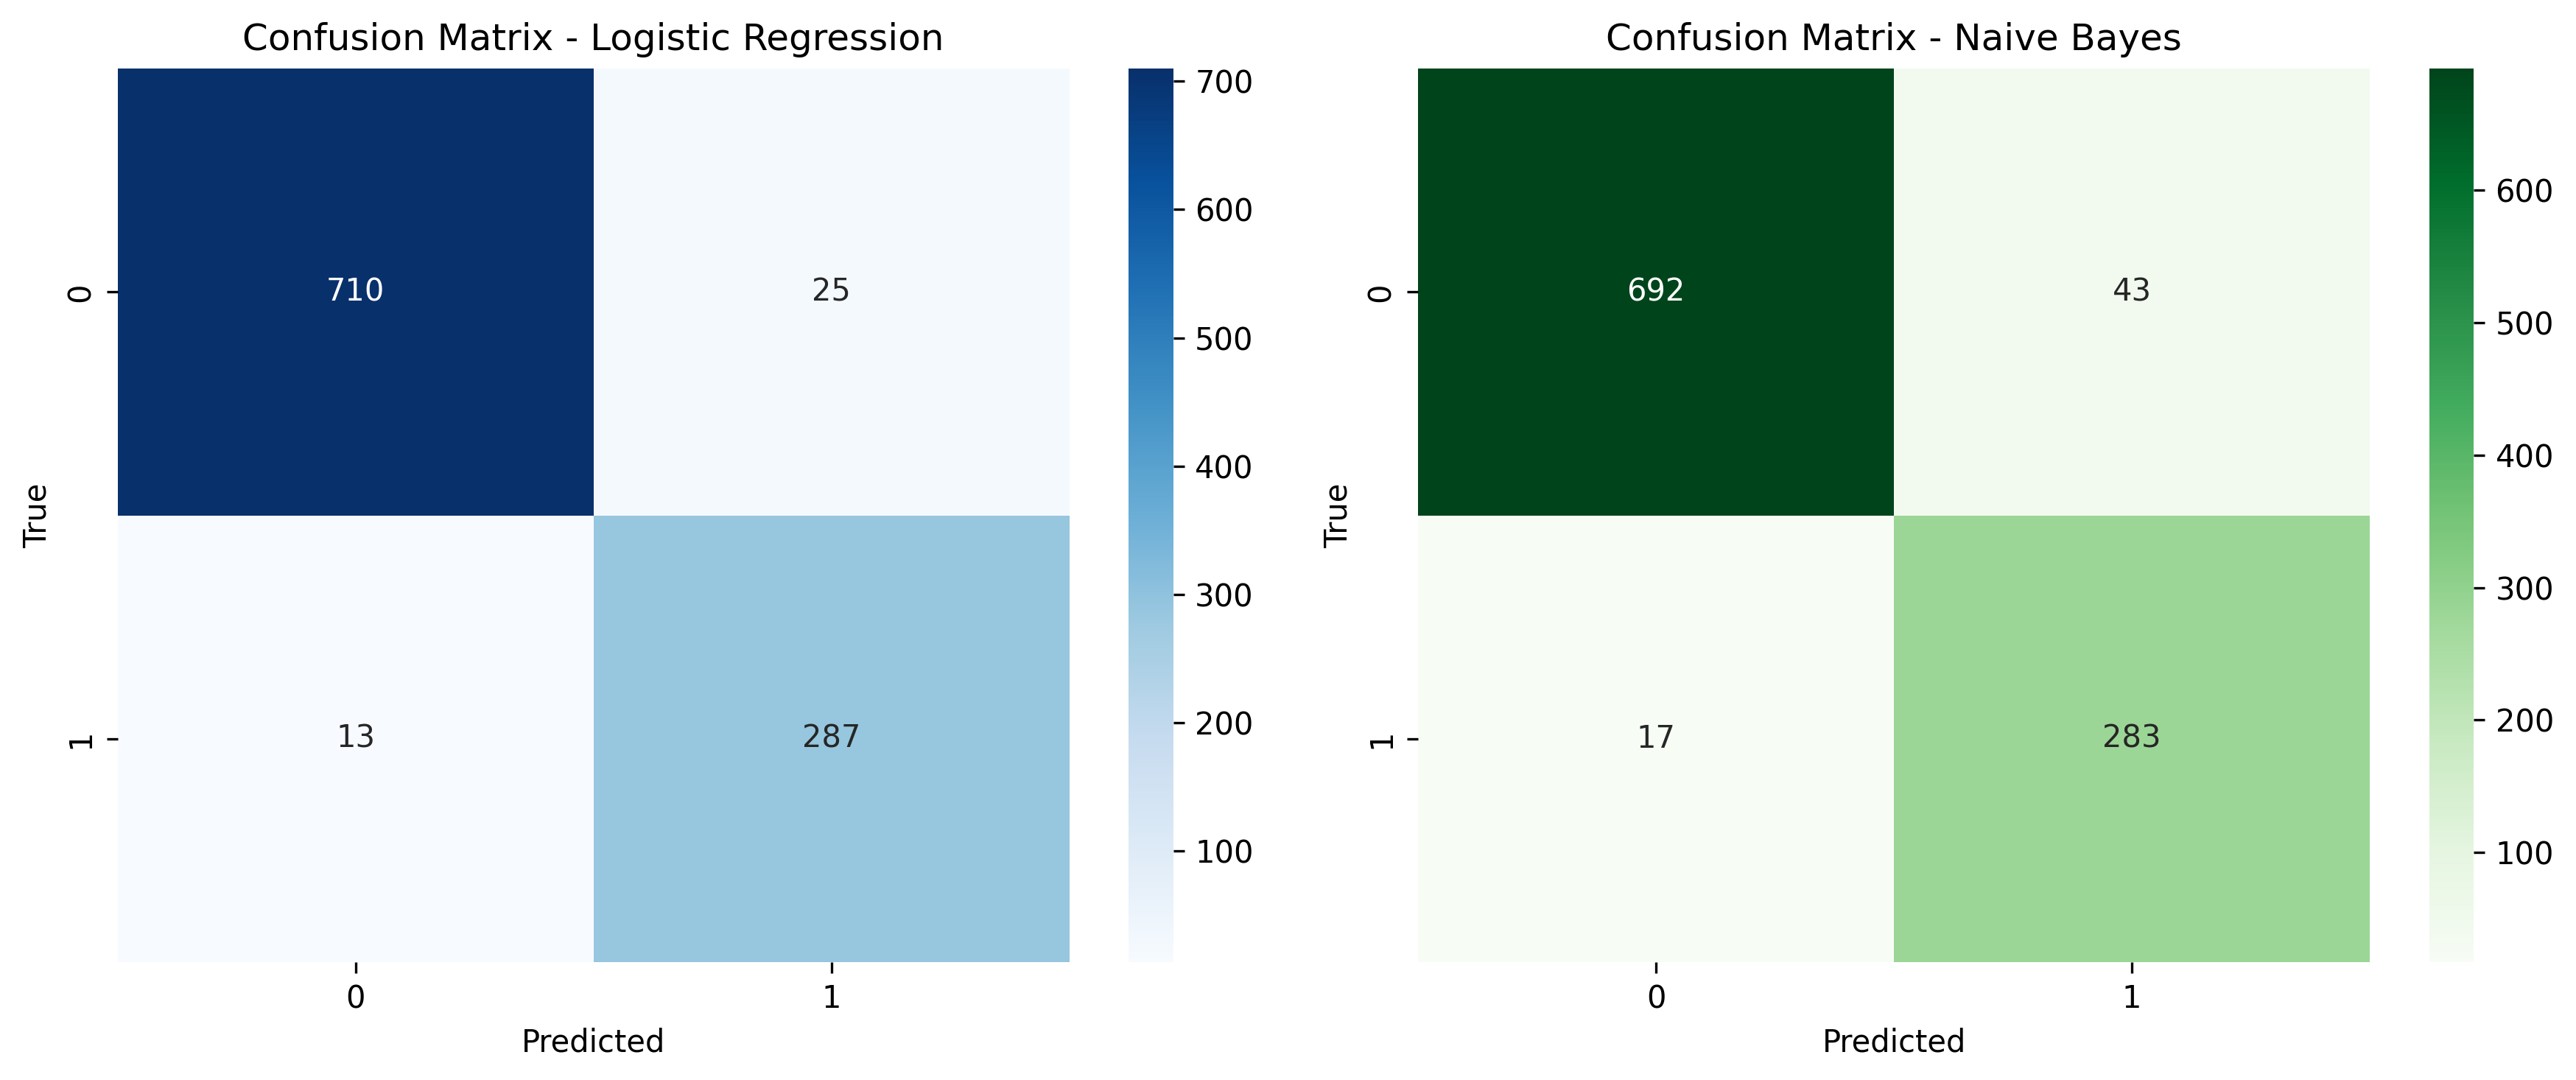
\includegraphics[width=0.48\textwidth]{figures/q1_confusion_matrices.png}
\caption{Confusion matrix comparison for Q1 models.}
\label{fig:q1-cm}
\end{figure}

Figure~\ref{fig:q1-cm} confirms the quantitative result: Logistic Regression provides a cleaner separation between positive and negative classes.

\begin{figure}[H]
\centering
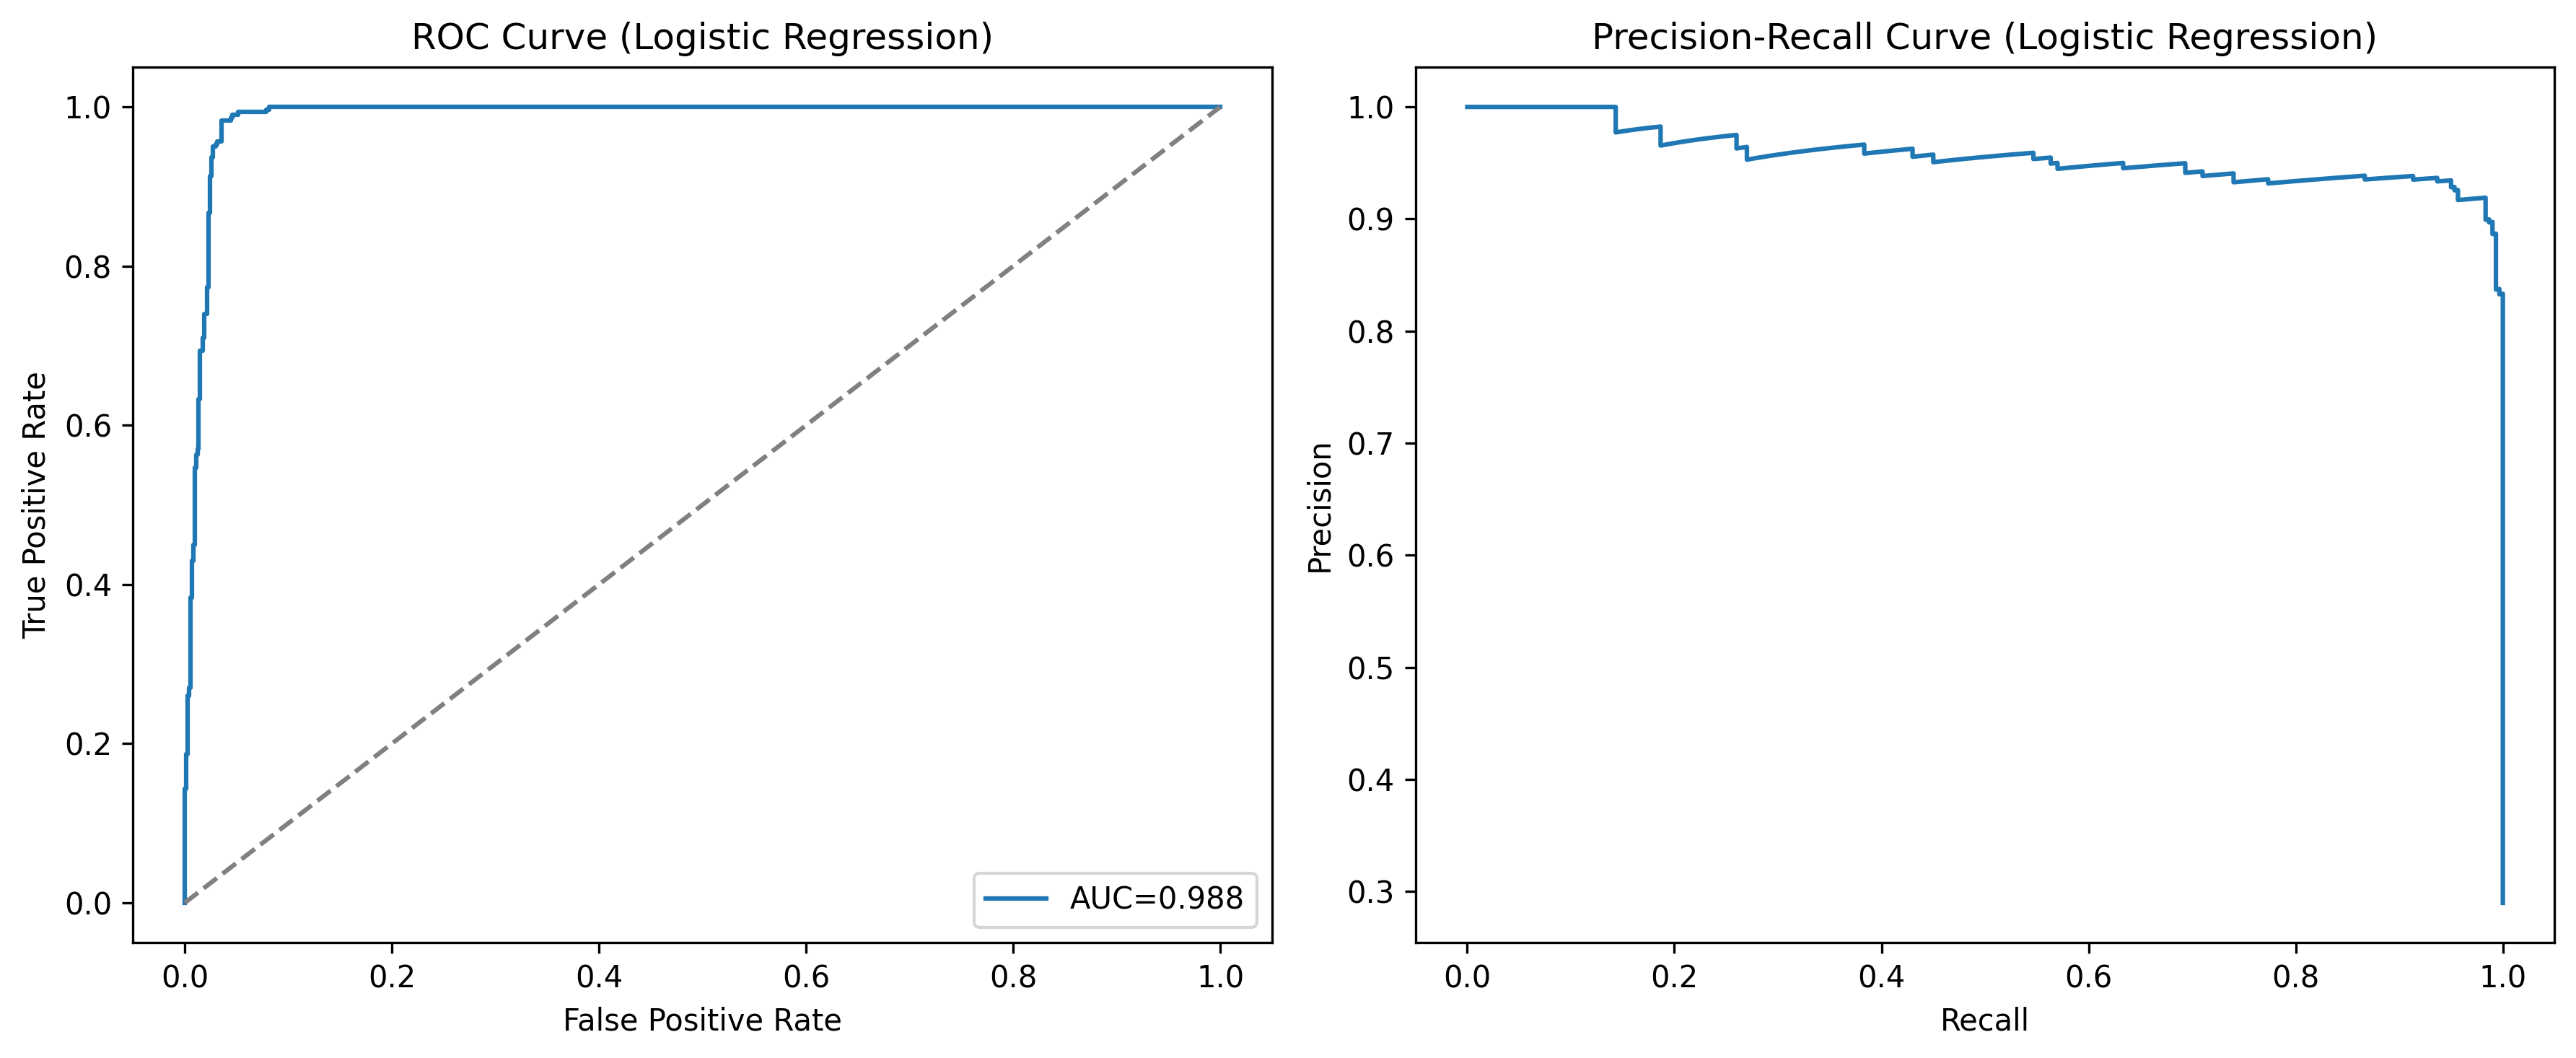
\includegraphics[width=0.48\textwidth]{figures/q1_roc_pr_curves_lr.png}
\caption{ROC and Precision-Recall curves for from-scratch Logistic Regression.}
\label{fig:q1-roc-pr}
\end{figure}

The ROC/PR visualization in Figure~\ref{fig:q1-roc-pr} demonstrates robust ranking quality and threshold flexibility, important for downstream tuning under varying business costs.

\subsection{Lexical Interpretation}

\begin{figure}[H]
\centering
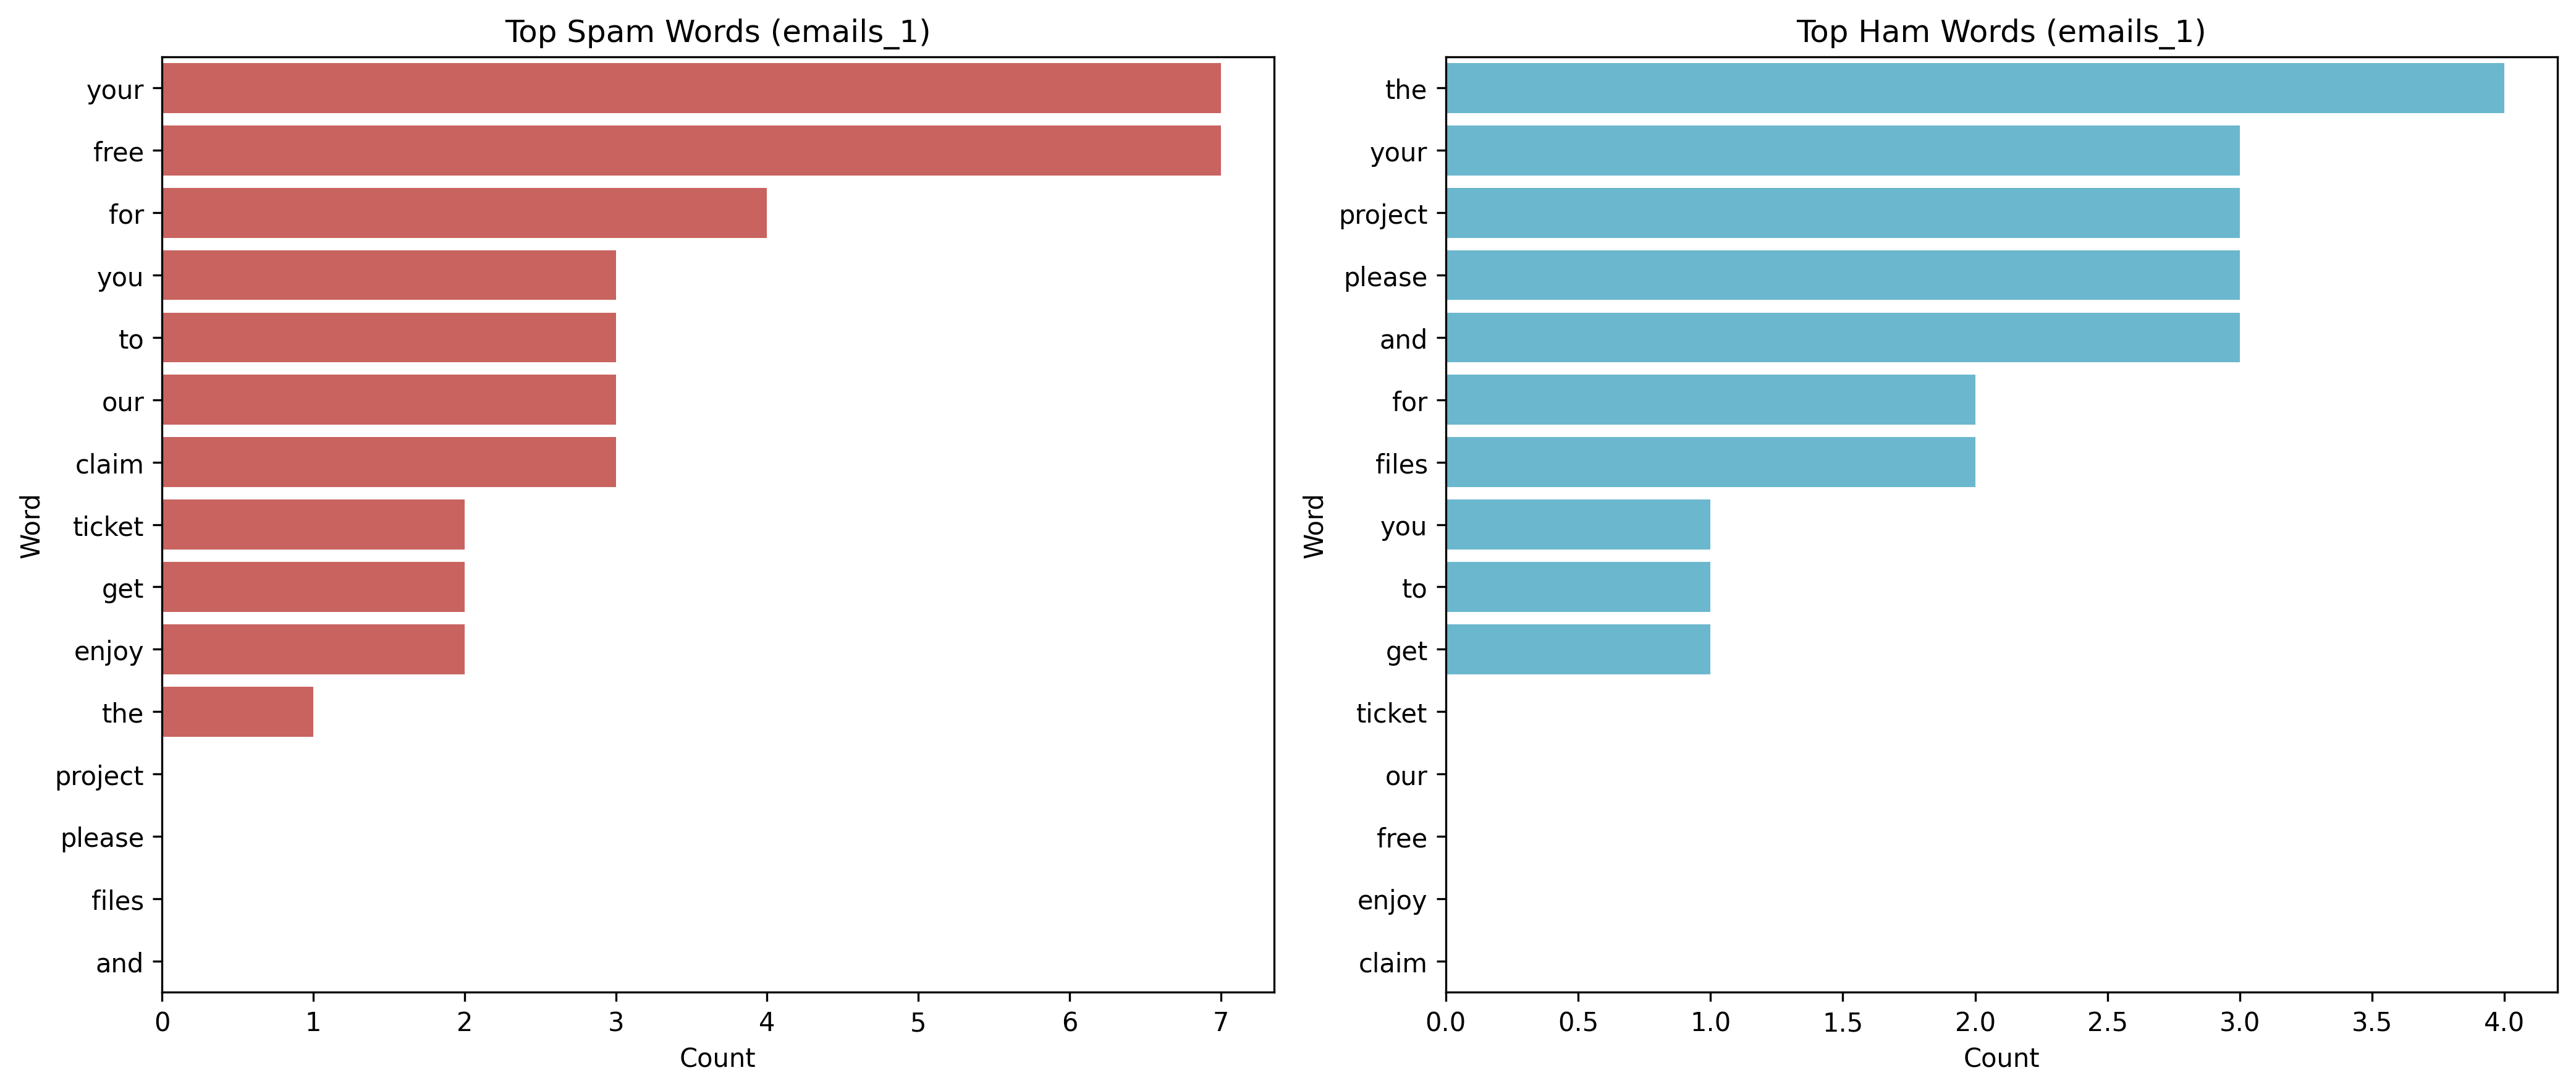
\includegraphics[width=0.48\textwidth]{figures/q1_top_words_spam_ham.png}
\caption{Top class-specific terms from the BoW projection of \texttt{emails\_1.csv}.}
\label{fig:q1-words}
\end{figure}

Figure~\ref{fig:q1-words} highlights class-discriminative lexical signals. Although this mini-dataset is not used for main model training, it helps validate preprocessing assumptions and demonstrates why token-frequency models remain competitive for spam filtering.

\begin{figure}[H]
\centering
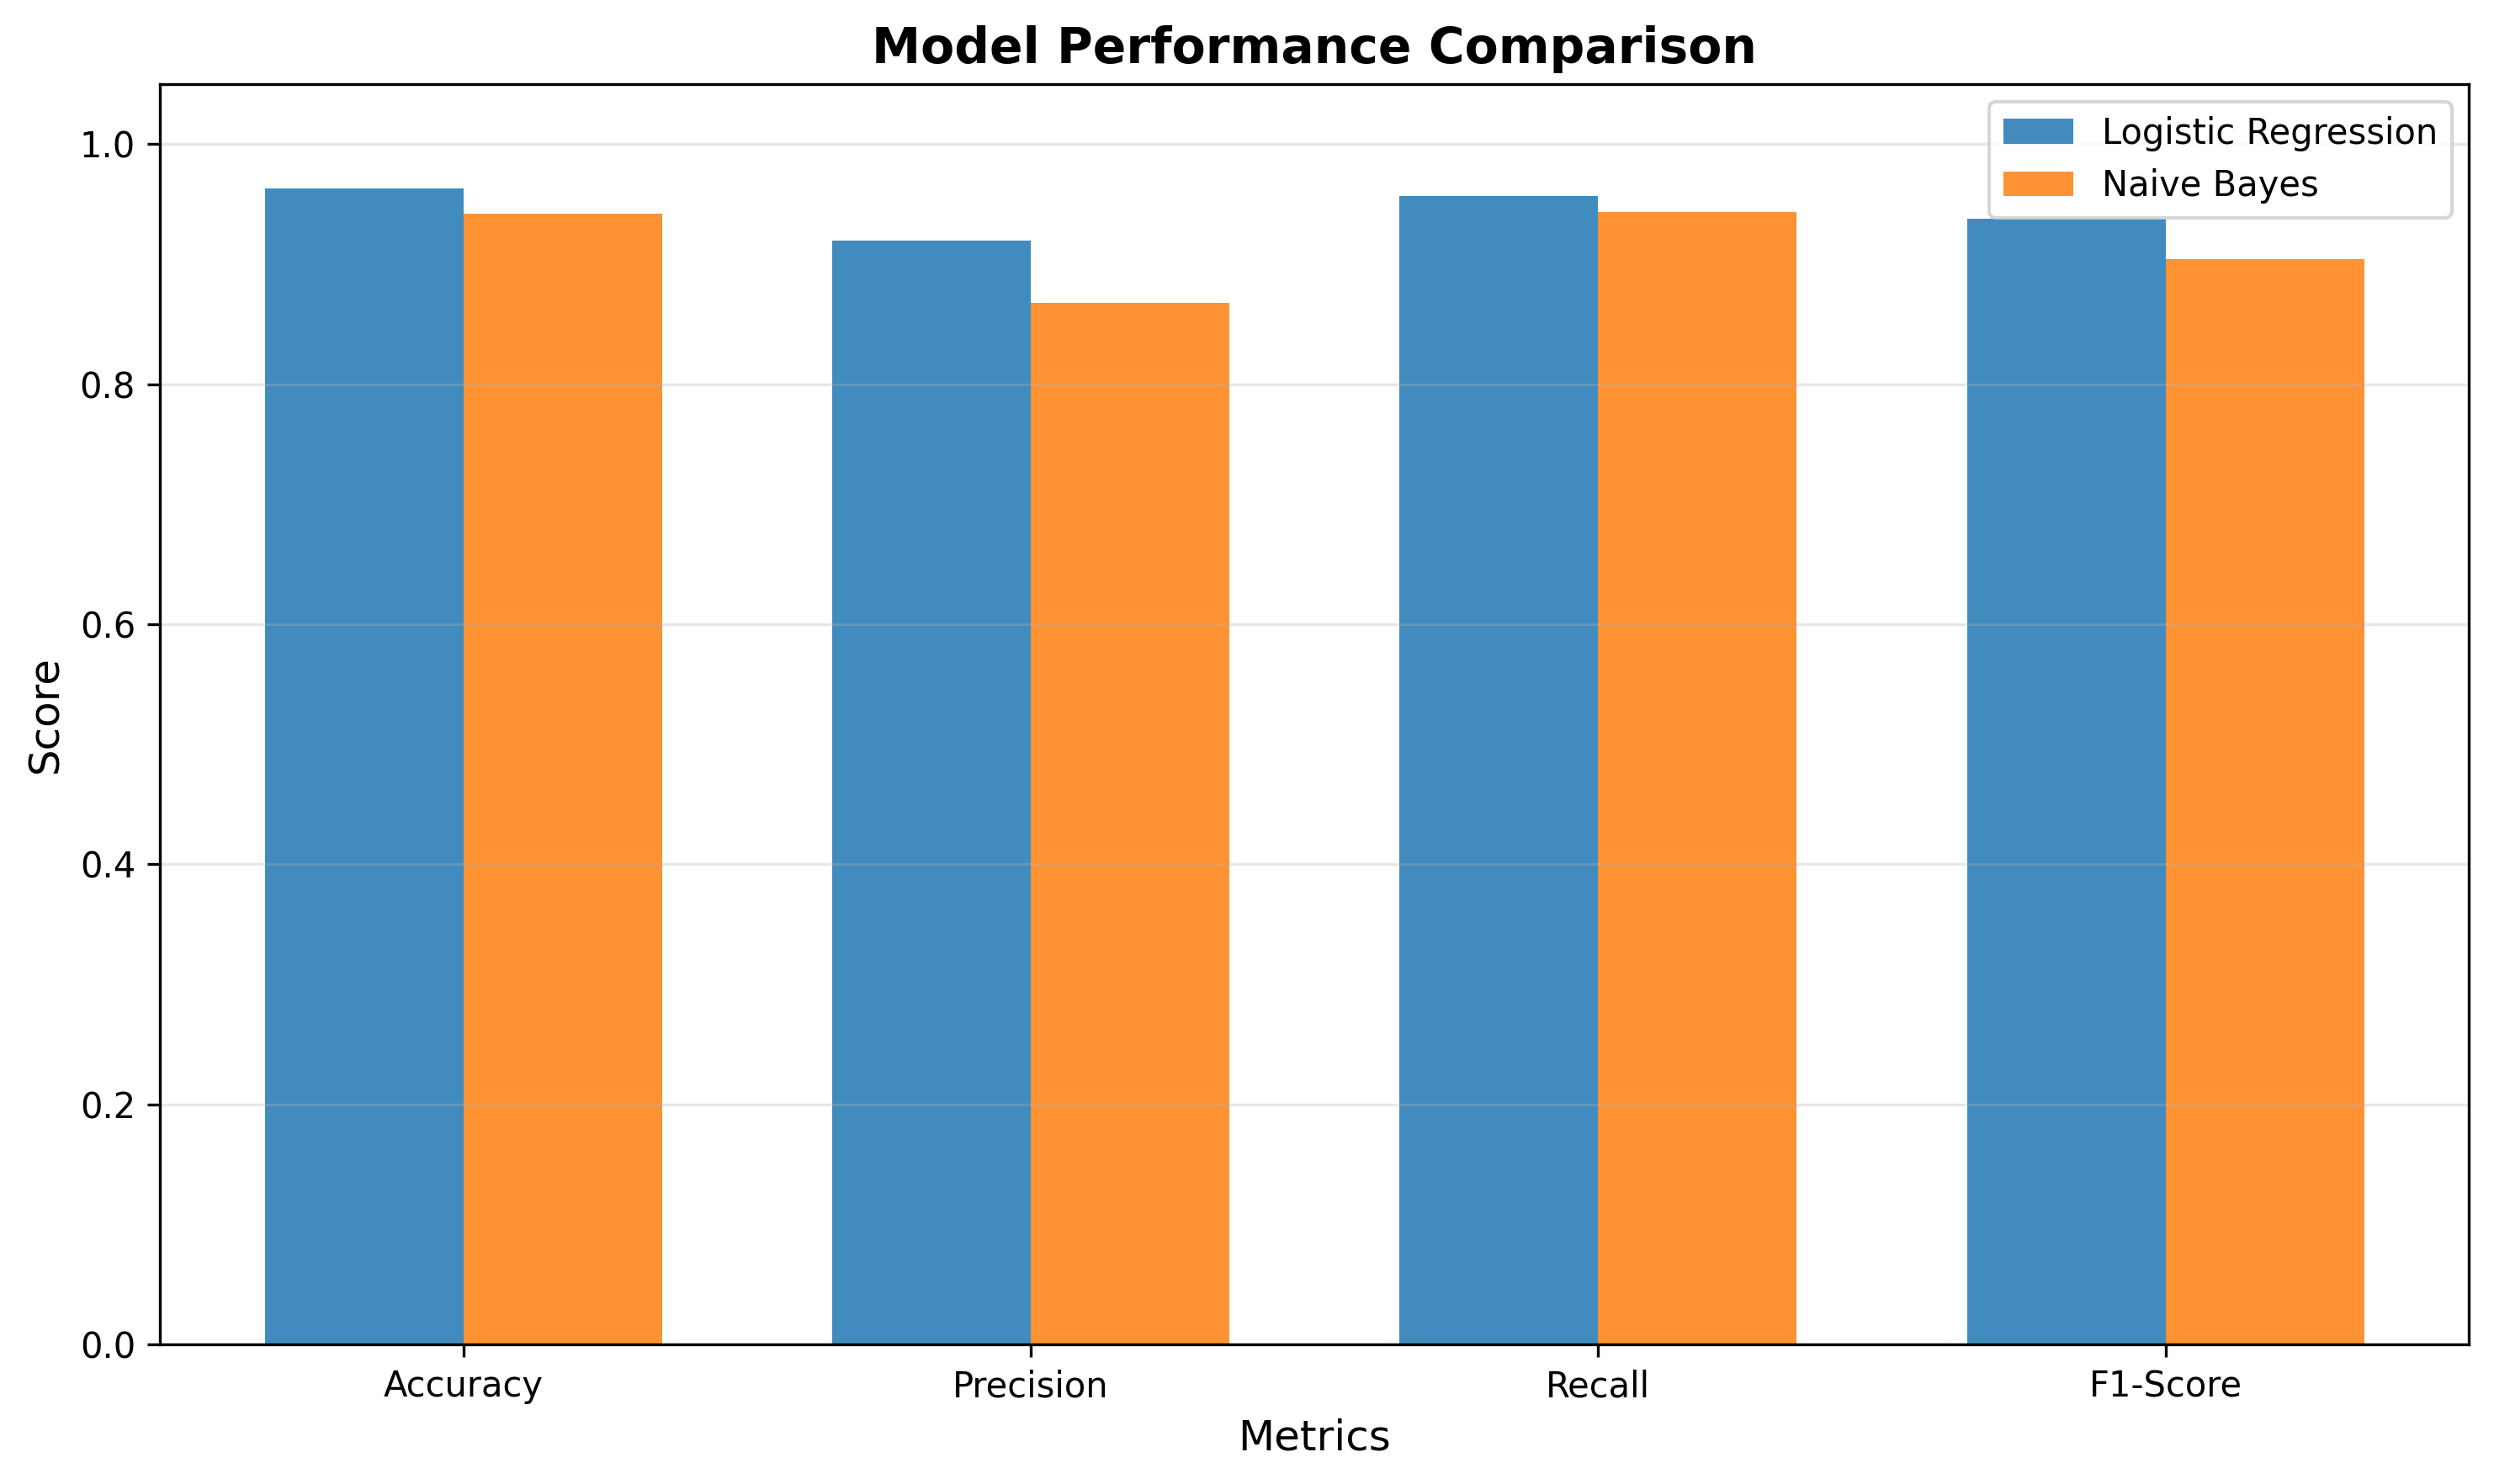
\includegraphics[width=0.48\textwidth]{figures/q1_model_comparison_bar.png}
\caption{Metric-level comparison for Q1 models.}
\label{fig:q1-bar}
\end{figure}

Figure~\ref{fig:q1-bar} summarizes model differences compactly and is consistent with the numerical table.

\subsection{Why Logistic Regression Wins Here}

Three factors explain the observed superiority of Logistic Regression:
\begin{enumerate}
    \item \textbf{Correlated lexical features:} words in real emails are not conditionally independent, violating Naive Bayes assumptions.
    \item \textbf{Discriminative optimization:} Logistic Regression optimizes a direct classification objective.
    \item \textbf{Feature normalization and gradient training:} stable optimization improves calibration on dense high-dimensional vectors.
\end{enumerate}

Naive Bayes still offers advantages in simplicity and training speed, but in this setting accuracy-oriented performance favors the discriminative model.
